\documentclass[12pt,a4paper]{report}
\usepackage[T2A]{fontenc}
\usepackage[utf8]{inputenc}
\usepackage[russian]{babel}
\usepackage{graphicx, setspace}
\usepackage{minted}

\usepackage[
top = 1.25cm, 
bottom = 2.0cm]{geometry}

\begin{document}
\begin{titlepage} 
	\centering
    % HEADER
	{
        \scshape
        Федеральное государственное автономное образовательное учреждение высшего образования
        \par
        \textbf{«Научно-образовательная корпорация ИТМО»}
        \par
        \vspace*{1cm}
        Факультет Программной Инженерии и Компьютерной Техники
        \par
    }
    % LOGO
    \vspace*{0.6cm}
    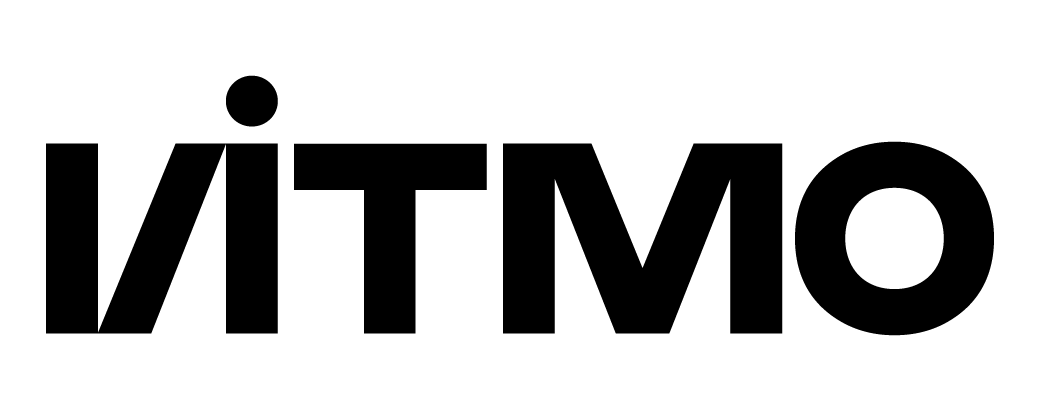
\includegraphics[width=\textwidth]{logo.png}
    % LAB INFO
    {
        \Large
        \textbf{Лабораторная работа по предмету \\ <<Системы ввода-вывода>> №2}
        \par
        \normalsize
        \vspace*{0.75cm}
        \textbf{Вариант 4}
        \par
    }
    \vfill
    % СREDITS
    \hfill\begin{minipage}{\dimexpr\textwidth-7.8cm}
        \textbf{Выполнил:}\par
        Степанов Арсений Алексеевич\par
        \vspace*{0.15cm}
        \textbf{Группа:}\par
        P3318 / СВВ 1.1\par
        \vspace*{0.15cm}
        \textbf{Преподаватель:}\par
        Табунщик Сергей Михайлович\par
    \end{minipage}
    \vfill
    Санкт-Петербург, \the\year{}г.
\end{titlepage}  
\section*{Цели работы}
Написать драйвер символьного устройства, удовлетворяющий
требованиям:
\begin{itemize}
    \item Должен создавать символьное устройство /dev/varN, где N – это
номер варианта
    \item Должен обрабатывать операции записи и чтения в соответствии с
вариантом задания
\end{itemize}
При записи текста в файл символьного устройства должен
осуществляться подсчет введенных цифр. Последовательность
полученных результатов (количество цифр) с момента
загрузки модуля ядра должна выводиться при чтении файла
\pagebreak
\section*{Выполнение}
Обработчик var4\_write предназначен для приёма данных из userspace, подсчёта количества цифровых символов в переданном буфере и
сохранения полученного результата во внутреннем динамическом массиве модуля. Для выполнения этой операции используется вспомогательная функция count\_digits\_in\_user\_buf, которая поэтапно копирует данные из пользовательской памяти в буфер ядра с помощью copy\_from\_user и подсчитывает количество символов в диапазоне от '0' до '9'. После получения результата функция var4\_write под защитой мьютекса results\_lock вызывает функцию append\_result, добавляющую вычисленное значение в массив результатов. Если текущей ёмкости массива недостаточно, в append\_result выполняется перевыделение памяти с помощью krealloc.

\subsubsection*{Код функции var4\_write}
\begin{minted}[fontsize=\small, frame=lines, linenos]{c}
static ssize_t var4_write(struct file *file, const char __user *buf,
                          size_t count, loff_t *ppos) {
  u32 digits;
  int ret;

  ret = count_digits_in_user_buf(buf, count, &digits);
  if (ret)
    return ret;

  mutex_lock(&results_lock);
  ret = append_result(digits);
  mutex_unlock(&results_lock);
  if (ret)
    return ret;

  return count;
}
\end{minted}

\subsubsection*{Код функции count\_digits\_in\_user\_buf}
\begin{minted}[fontsize=\small, frame=lines, linenos]{c}
static int count_digits_in_user_buf(const char __user *buf, size_t count,
                                    u32 *out) {
  char chunk[256];
  size_t copied = 0;
  u32 digits = 0;
  size_t i;

  while (copied < count) {
    size_t to_copy = min(sizeof(chunk), count - copied);

    if (copy_from_user(chunk, buf + copied, to_copy))
      return -EFAULT;

    for (i = 0; i < to_copy; i++) {
      if (chunk[i] >= '0' && chunk[i] <= '9')
        digits++;
    }

    copied += to_copy;
  }

  *out = digits;
  return 0;
}
\end{minted}

\subsubsection*{Код функции append\_result}
\begin{minted}[fontsize=\small, frame=lines, linenos]{c}
static int append_result(u32 value) {
  size_t new_capacity;
  u32 *new_results;

  if (results_count == results_capacity) {
    new_capacity = results_capacity ? (results_capacity * 2) : 16;
    new_results =
        krealloc(results, new_capacity * sizeof(*results), GFP_KERNEL);
    if (!new_results)
      return -ENOMEM;

    results = new_results;
    results_capacity = new_capacity;
  }

  results[results_count++] = value;
  return 0;
}
\end{minted}
Обработчик var4\_read предназначен для передачи пользователю всех ранее накопленных результатов. Сначала под защитой мьютекса создаётся снимок текущего массива результатов с помощью kmemdup, что позволяет минимизировать время удержания блокировки. Далее вычисляется необходимый размер текстового представления всех чисел; для этого используется вспомогательная функция u32\_dec\_len, определяющая количество десятичных цифр в каждом значении типа u32. После выделения памяти функцией kmalloc формируется текстовый буфер, в который результаты записываются построчно с помощью scnprintf. Готовые данные копируются в пользовательское пространство через simple\_read\_from\_buffer, после чего вся временно выделенная память освобождается функцией kfree.

\subsubsection*{Код функции var4\_read}
\begin{minted}[fontsize=\small, frame=lines, linenos]{c}
static ssize_t var4_read(struct file *file, char __user *buf, size_t count,
                         loff_t *ppos) {
  u32 *snapshot;
  size_t snapshot_count;
  size_t i;
  size_t text_len = 0;
  char *text;
  size_t pos = 0;
  ssize_t ret;

  mutex_lock(&results_lock);
  snapshot_count = results_count;
  if (snapshot_count == 0) {
    mutex_unlock(&results_lock);
    return 0;
  }

  snapshot = kmemdup(results, snapshot_count * sizeof(*results), GFP_KERNEL);
  mutex_unlock(&results_lock);
  if (!snapshot)
    return -ENOMEM;

  for (i = 0; i < snapshot_count; i++)
    text_len += u32_dec_len(snapshot[i]) + 1;

  text = kmalloc(text_len + 1, GFP_KERNEL);
  if (!text) {
    kfree(snapshot);
    return -ENOMEM;
  }

  for (i = 0; i < snapshot_count; i++)
    pos += scnprintf(text + pos, text_len + 1 - pos, "%u\n", snapshot[i]);

  ret = simple_read_from_buffer(buf, count, ppos, text, text_len);

  kfree(text);
  kfree(snapshot);
  return ret;
}
\end{minted}
\subsection*{Результаты работы модуля}
\begin{center}
    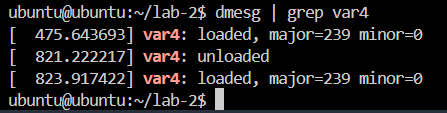
\includegraphics{assets/image.png}
\end{center}
\begin{center}
    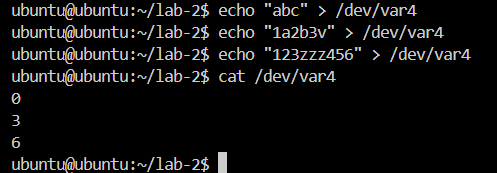
\includegraphics{assets/logs.png}
\end{center}
\section*{Выводы}
Я научился работать с модулями ядра Linux и написал драйвер блочного
устройства, которое поддерживает операции чтения/записи и обработку
полученных данных
\end{document}
